\documentclass[11pt,xcolor=svgnames]{beamer}
\usepackage{dsfont,natbib,setspace,changepage,multirow}
\mode<presentation>

% replaces beamer foot with simple page number
\setbeamertemplate{navigation symbols}{}
\setbeamerfont{frametitle}{series=\bfseries,size=\normalsize}
\setbeamercolor{frametitle}{fg=Black}

\setbeamertemplate{footline}{
   \raisebox{5pt}{\makebox[\paperwidth]{\hfill\makebox[20pt]{\color{gray}\scriptsize\insertframenumber}}}}

\usepackage{algorithm}
\usepackage{algorithmic}

% colors
\newcommand{\theme}{\color{DarkBlue}}
\newcommand{\bk}{\color{black}}
\newcommand{\rd}{\color{red}}
\newcommand{\fg}{\color{ForestGreen}}
\newcommand{\bl}{\color{blue}}
\newcommand{\gr}{\color{black!50}}
\newcommand{\sg}{\color{DarkSlateGray}}
\newcommand{\nv}{\color{Navy}}
\setbeamercolor{itemize item}{fg=gray}

% common math markups
\newcommand{\bs}[1]{\boldsymbol{#1}}
\newcommand{\mc}[1]{\mathcal{#1}}
\newcommand{\mr}[1]{\mathrm{#1}}
\newcommand{\bm}[1]{\mathbf{#1}}
\newcommand{\ds}[1]{\mathds{#1}}
\newcommand{\indep}{\perp\!\!\!\perp}
\def\plus{\texttt{+}}
\def\minus{\texttt{-}}

% spacing and style shorthand
\setstretch{1.1}

\begin{document}

\setcounter{page}{0}
\begin{frame}[plain]
\begin{center}

{\bf \Large  Scalable Semiparametrics for Fat Tails}

\vskip 1cm \large
Matt Taddy -- {\tt http://taddylab.com}

\vskip .1cm
{ Microsoft Research and Chicago Booth}

\vskip .5cm
with Hedibert Lopes (Insper) and Matt Gardner (eBay)

\vskip .1cm  {\gr paper is at {\tt http://arxiv.org/abs/1602.08066}}

\end{center}
\end{frame} 


\begin{frame}

{\bf Big Data}

\vskip .25cm

\vskip .25cm
{\nv The sample sizes are enormous.}
\begin{itemize}
\item We'll see 21 and 200 million today.  
\item Data can't fit in memory, or even storage, on a single machine.
%\item Our familiar MCMC algorithms take too long.
\end{itemize}


\vskip .25cm
{\nv The data are super weird.  }
\begin{itemize}
\item Internet transaction data distributions have a big spike at zero and spikes at other discrete values (e.g., 1 or \$99).
\item Big tails (e.g., \$12 mil/month eBay user spend) that matter.
\item The potential feature space is unmanageably large.
\item We cannot  write down or measure believable models.
\end{itemize}

\vskip .5cm\theme
Both `Big' and `Strange' beg for nonparametrics.

\end{frame}

\begin{frame}

{\bf Distribution-free Bayesian nonparametrics}

\vskip .5cm
{Find some {\it statistic of the DGP} that you care about:}
\vskip .1cm
\begin{itemize}
\item derive from first principles, e.g. moment conditions
\item {\it an algorithm} that we know works, e.g. CART
\item think about geometric projections, e.g. OLS
\end{itemize}
\vskip .1cm
Call this statistic $\bs{\theta}(g)$ where $g(\bm{z})$ is the DGP (e.g., for $\bm{z} = [\bm{x},y]$).

\vskip .5cm
Then you write down a flexible  model for the DGP $g$, and study properties of the posterior on $\bs{\theta}(g)$ induced by the posterior over $g$.

\end{frame}

\begin{frame}

{\bf A flexible model for the DGP}

\vskip .5cm
Say $\bm{z} = [\bm{x},y]$ is a single {\it independent} data point.

\vskip .25cm Each data point assumes one of a {\it finite} number of possible values, $[\bs{\zeta}_1 \ldots \bs{\zeta}_L]$, with probabilities proportional to $[\bs{\theta}_1 \ldots \bs{\theta}_L]$.
\begin{equation*}
g(\bm{z}) = \frac{1}{|\bs{\theta}|}\sum_{l=1}^L \theta_l \ds{1}_{[\bm{z} =
\bs{\zeta}_l]}\end{equation*}

We complete specification with a conjugate prior on the weights:
\[\frac{\bs{\theta}}{|\bs{\theta}|} \sim \mr{Dir}(a) \propto \frac{1}{|\bs{\theta}|^{L(a-1)}}\prod_l \theta_l^{a-1}~~\text{where}~~a,\theta_l >0.
\]
%The support is treated as fixed.

%\vskip .25cm
This is the Dirichlet-multinomial sampling model {\gr (Ferguson 1973)}.  

\end{frame}

\begin{frame}

Now you've observed some data, say $\bm{Z} = \{\bm{z}_1 \ldots \bm{z}_n\}$.\\
{\gr (say every $\bm{z}_i = [\bm{x}_i,y_i]$ is unique)}.

\vskip .25cm
The posterior over weights has $\theta_l \stackrel{ind}{\sim} \mr{Exp}\left(a+\ds{1}_{[\bs{\zeta}_l \in \bm{Z}]}\right)$. 

\vskip .5cm
{\bf A convenient limiting case}

\vskip .25cm
$a \to 0$ leads to $\mr{p}(\theta_l = 0) = 1$ for $\bs{\zeta}_l \notin \bm{Z}$.

\vskip .2cm
In this case, we can focus on only the {\it observed support} and write the posterior for our DGP
\[
g(\bm{z}) = \tfrac{1}{|\bs{\theta}|}
\sum_{i=1}^n \theta_i \ds{1}{[\bm{z} =
\bm{z}_i]},~~~\theta_i \stackrel{iid}{\sim} \mr{Exp}(1).
\]

\hfill
{This is just the Bayesian bootstrap. \gr (Rubin 1981)}

\end{frame}


% \begin{frame}

% \vskip .25cm
% Recall your early stats: {\theme the sampling distribution.}

% \vskip .1cm
% Imagine getting multiple datasets of size $n$ from the population.

% \vskip .1cm
% The {\it sampling distribution} of an estimator $\hat \beta$\\ is
% the histogram of your estimates for each dataset.


% \vskip .25cm
% 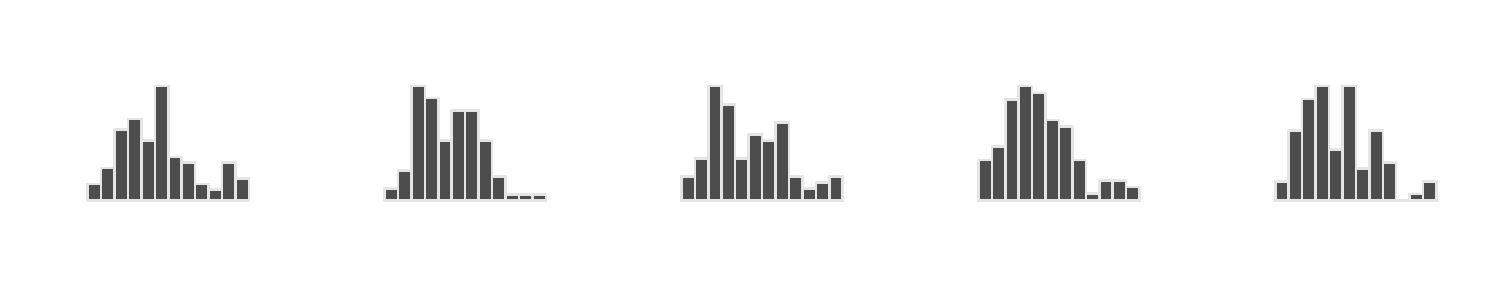
\includegraphics[width=4.2in]{graphs/bs_boothist}

% \vskip -.2cm
% $
% ~\begin{array}{c}\downarrow\\
%     \hat\beta_1\\
%     ~~\searrow
% \end{array}
% $
% \hskip 1.1cm
% $
% \begin{array}{c}\downarrow\\
%     \hat\beta_2\\
%     ~~\searrow
% \end{array}
% $
% \hskip 1.1cm
% $
% \begin{array}{c}\downarrow\\
%     \hat\beta_3\\
%     \downarrow
% \end{array}
% $
% \hskip 1.1cm
% $
% \begin{array}{c}\downarrow\\
%     \hat\beta_4\\
%     \swarrow~~
% \end{array}
% $
% \hskip 1.1cm
% $
% \begin{array}{c}\downarrow\\
%     \hat\beta_5\\
%     \swarrow~~
% \end{array}
% $

% \begin{center}
% 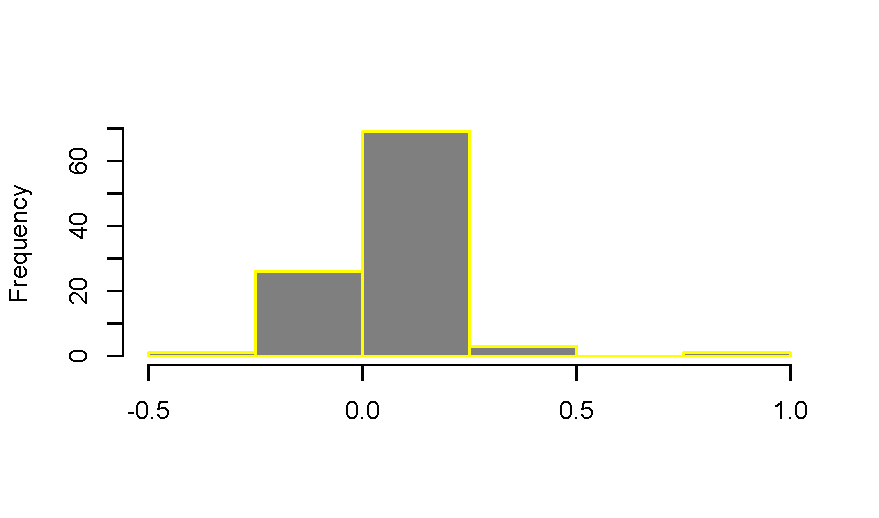
\includegraphics[width=2.25in]{graphs/boothist}
% \end{center}
 

% \vskip -.5cm
% \end{frame}

% \begin{frame}


% {\bf \theme The Bootstrap:} resample your data {\it with replacement} \\
% ~~~~~~~~~~~~~~~~~~ and calculate  some statistic of interest.  

% \vskip .1cm {\it \gr With-Replacement: each draw is put back in the `bucket', so it is possible to sample the same
% observation multiple times.  }

% \vskip .5cm
% To raise oneself up by bootstraps...  
% {\gr (Try it; it doesn't work).}

% \vskip .05cm    The metaphor refers
% to surprising examples of self sufficiency.

% \vskip .5cm
% For $b=1\ldots B$ `bootstrap samples'
% \begin{itemize}\nv
% \item Resample {\theme with replacement} $n$ observations.
% \item Calculate your estimate (e.g., $\hat\beta_b$).
% \end{itemize}

% \vskip .5cm
% This is an {\it approximation} to the sampling distribution.

% \vskip .1cm
% For example, an approx SE($\hat\beta$) is
% $\mr{sd}(\hat\beta) =\sqrt{\frac{1}{B}
% \sum_b (\hat \beta_b - \bar{\beta})^2}.
% $

% \end{frame}


% \begin{frame}

% {\bf \theme The Bootstrap: \bk why it works}

% \begin{center}
% 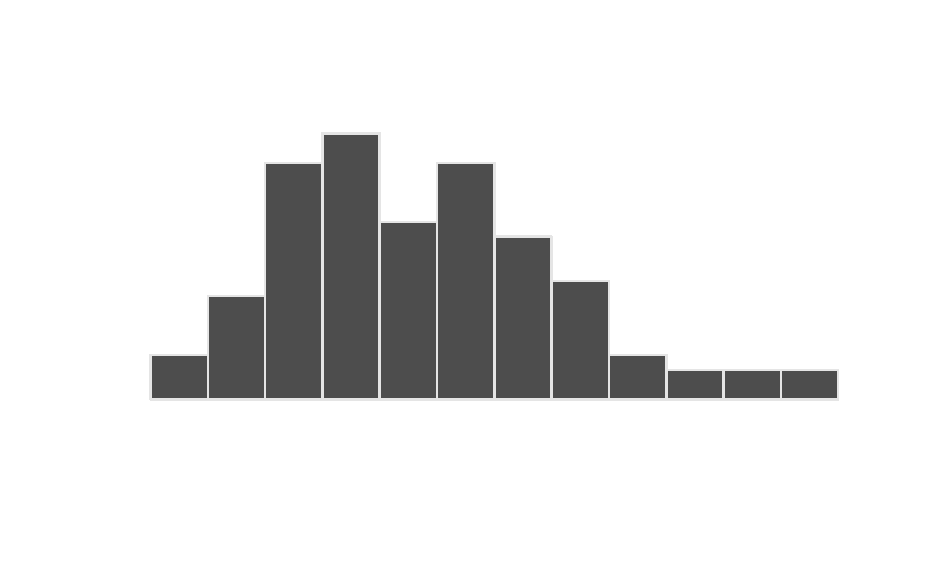
\includegraphics[width=2in]{graphs/bs_bighist}

% {\gr data sample}

% $\swarrow~~~\downarrow~~~\searrow$

% 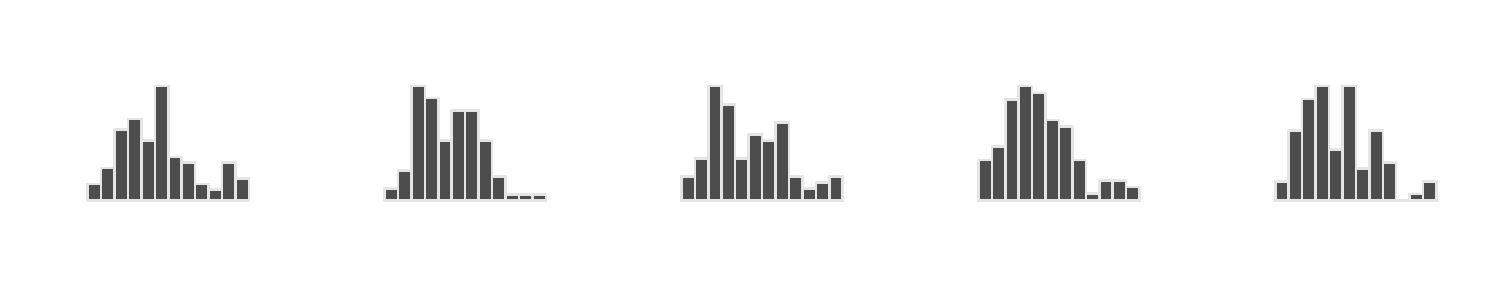
\includegraphics[width=4.25in]{graphs/bs_boothist}

% \gr bootstrap samples
% \end{center}

% You are pretending that the {\it empirical data distribution} is
% the population, and using it to draw alternative samples.
% \end{frame}



% \begin{frame}

% {\bf The {\nv Bayesian} Bootstrap}

% \begin{center}
% 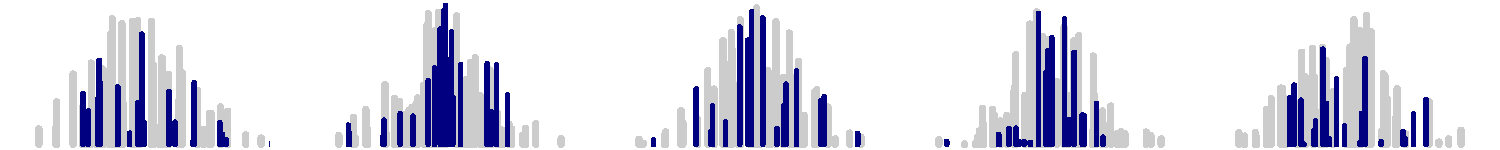
\includegraphics[width=\textwidth]{graphs/bayesbootprior}

% {\gr prior samples}

% $\downarrow~~~~\downarrow~~~~\downarrow$

% 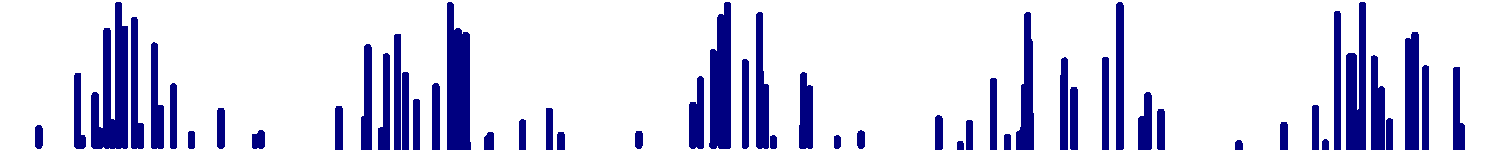
\includegraphics[width=\textwidth]{graphs/bayesbootpost}

% \gr posterior samples
% \end{center}

% You have a nonparametric model over {\it all} possible observations, but then
% use a convenient prior that limits you to observed support.

% \vskip .5cm
% It'll work whenever the standard Bootstrap works: only if the empirical data distribution 
% is a decent substitute for the population.

% \end{frame}

% z <- x <- c()
% dz <- dx <- c()
% for(i in 1:5){
%  x <- cbind(x,rnorm(20))
%  z <- cbind(z,rnorm(50))
%  dx <- cbind(dx,dnorm(x[,i])*runif(20))
%  dz <- cbind(dz,dnorm(z[,i])*runif(50))}

% pdf("graphs/bayesbootprior.pdf",width=10,height=1)
% par(mai=c(0,.2,0,.2),mfrow=c(1,5))
% for(i in 1:5){
%  plot(z[,i],dz[,i],type="h",col="grey80",ylim=c(0,max(c(dx,dz))),
%   xaxt="n",yaxt="n", bty="n",lwd=4,xlab="",ylab="")
%  lines(x[,i],dx[,i],type="h",col="navy",lwd=3)}
% dev.off()

% z <- x <- c()
% dz <- dx <- c()
% for(i in 1:5){
%  x <- cbind(x,rnorm(20))
%  z <- cbind(z,rnorm(50))
%  dx <- cbind(dx,dnorm(x[,i])*runif(20))
%  dz <- cbind(dz,dnorm(z[,i])*runif(50))}

% pdf("graphs/bayesbootpost.pdf",width=10,height=1)
% par(mai=c(0,.2,0,.2),mfrow=c(1,5))
% for(i in 1:5)
%     plot(x[,i],dx[,i],type="h",col="navy",
%      xaxt="n",yaxt="n", bty="n",lwd=4,xlab="",ylab="")
% dev.off()

\begin{frame}

{\bf {\gr Example: } Ordinary Least Squares}

\vskip .5cm
{\it Population} OLS is a posterior functional
\begin{equation*}
\bs{\beta} = (\bm{X}'\bs{\Theta}\bm{X})^{-1}  \bm{X}'\bs{\Theta}\bm{y}
\end{equation*}
where $\bs{\Theta} = \mr{diag}(\bs{\theta})$.  
{\theme This is a random variable. \gr (sample via BB)}

\vskip .75cm
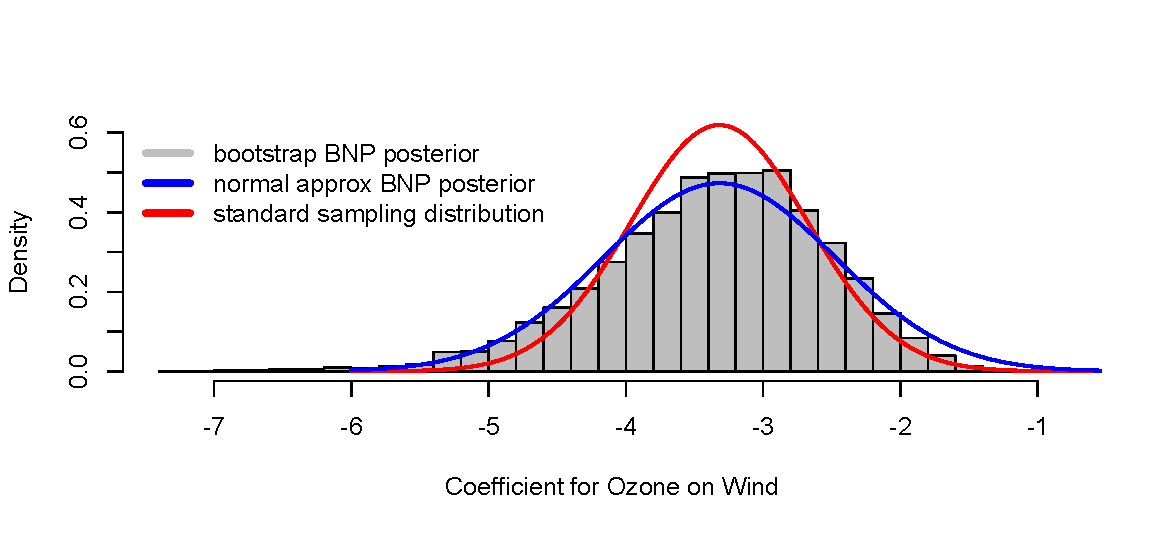
\includegraphics[width=\textwidth]{graphs/ozone}
\end{frame}

% \begin{frame}[fragile]

% {\footnotesize\gr
% \begin{verbatim}
% data(airquality); n <- nrow(airquality)
% B <- 1000; beta <- vector(length=B)
% for(b in 1:B){
%   fit <- lm(Ozone ~., data=airquality, weights=rexp(n))
%   beta[b] <- coef(fit)["Wind"] }
% sampfit <- lm(Ozone ~ ., data=airquality)
% coef <- summary(sampfit)$coef["Wind",1:2]
% x <- as.matrix(cbind(1,na.omit(airquality)[,-1]))
% xxi <- solve(crossprod(x))
% sandwich <- xxi%*%t(x)%*%diag(sampfit$resid^2)%*%x%*%xxi
% hist(beta, col=8, main="", 
%   xlab="Coefficient for Ozone on Wind", 
%   freq=FALSE,ylim=c(0,0.6),breaks=25)
% grid <- seq(-6,5,length=500)
% lines(grid, dnorm(grid,coef[1],coef[2]),col=2,lwd=2)
% lines(grid, dnorm(grid,coef[1],sqrt(sandwich[3,3])),col=4,lwd=2)
% legend("topleft",col=c(8,2),lwd=4, 
%   legend=c("bootstrap BNP posterior",
%            "normal approx BNP posterior",
%            "standard sampling distribution"),bty="n")
% \end{verbatim}
% }

% \end{frame}




\begin{frame}

We've had a bunch of success with this strategy (and especially, taking advantage of analytic approximations to the BNP posterior).

\begin{itemize}
\item Bayesian forest alternative to Random Forests, and the scalable Empirical BF  {\gr (T, Chen, Yu, Wyle  2015 ICML)}
\item BNP theory for regression adjustement in treatment effect estimation  {\gr (T, Gardner, Chen, Draper 2016 JBES) }
\item BFs for heterogeneous treatment effects {\gr (T+ 2016 JBES)}
\end{itemize}

\vskip .25cm
But, at heart, we are essentially [nonparametric] bootstrapping.  
And sometimes the bootstrap fails: \\~~~~~e.g., model selection, high dimensions, and {\color{Maroon} heavy tails}.

\end{frame}


\begin{frame}


Internet transaction data is super heavy tailed.

\vskip .5cm
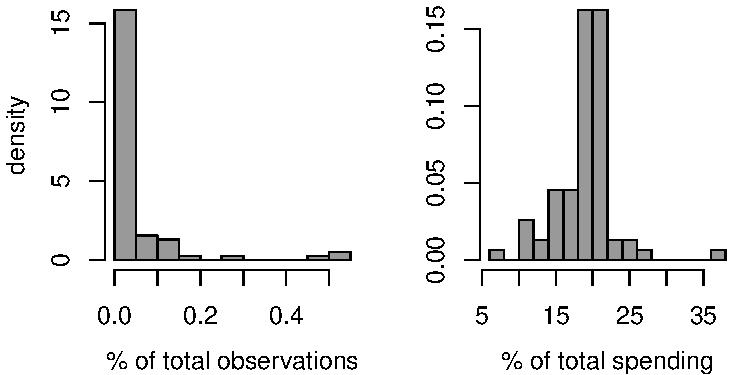
\includegraphics[width=.9\textwidth]{graphs/gt2k_proportion.pdf}

\vskip .25cm
The standard bootstrap fails for infinite variance distributions.  

\vskip .25cm
We should suspect our Bayesian bootstrap will have similarly bad frequentist properties.  {\color{Maroon} e.g., the posterior will not be consistent.}
\end{frame}

\begin{frame}
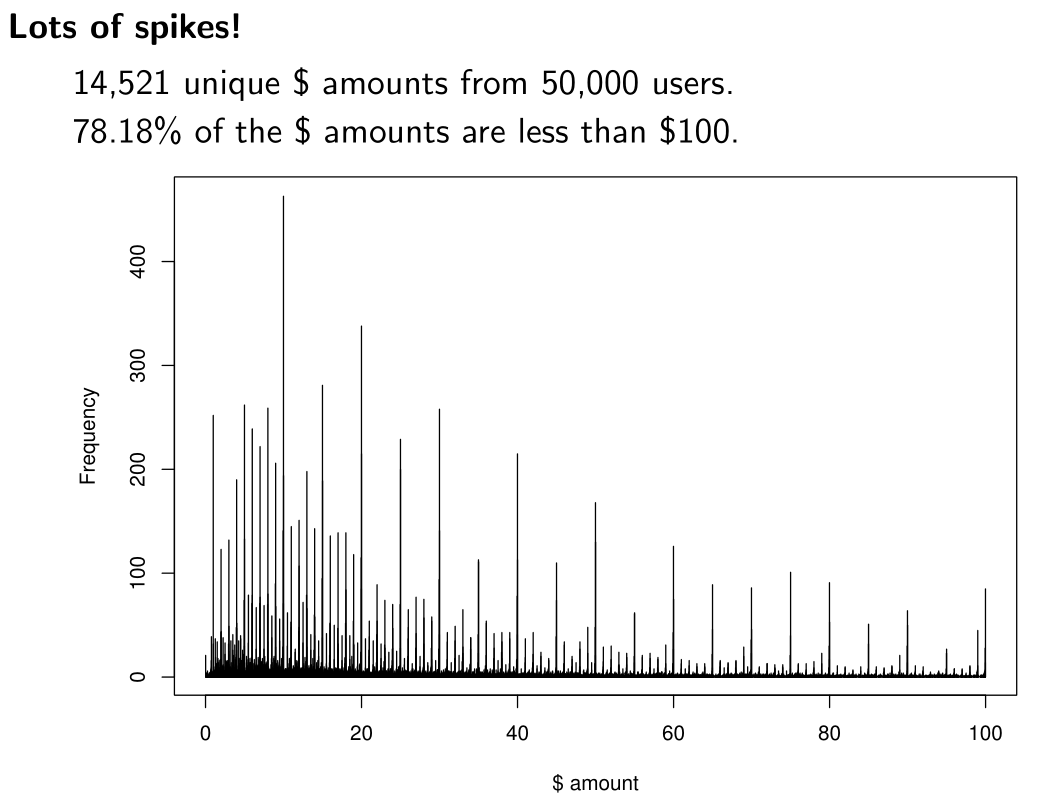
\includegraphics[width=.95\textwidth]{graphs/spikes.PNG}\\ \hfill
So the distribution below the tail is also screwy.
\end{frame}

\begin{frame}

{\bf Semi-parametrics: \theme only model where you really need it.}

\vskip .5cm
Add a parametric tail above some threshold $u$:
\[
\mr{p}(z ) = \frac{1}{|\bs{\theta}|}
\sum_{l=1}^L \theta_l \ds{1}{[z =
\zeta_l]} + \frac{\theta_{L+1}}{|\bs{\theta}|} \theme \mathrm{GPD}(z-u;~\xi,~\sigma)\ds{1}{[z \geq u]}
\]
where $\mathrm{GPD}$ is the generalized Pareto  $\mr{p}(y) = \frac{1}{\sigma}\left( 1 + \xi \frac{y}{\sigma}\right)^{-(\frac{1}{\xi} + 1)}$.

\vskip .5cm
A nice simple prior is $\pi(\sigma,\xi) = \frac{1}{\sigma}\xi^{a-1}(1-\xi)^{b-1}\mathds{1}_{\xi \in (0,1)}$.  

\vskip .2cm You can set $a = b = 1$ with enough data, but it is cooler to use background info.  {\color{Maroon} It is usually a bad idea to add information on $\sigma$.}

\end{frame}

\begin{frame}
{Inference}

Say $\mu = \ds{E}[z]$ and $\lambda = \ds{E}[z-u|z\geq u]$. 

\vskip .1cm
 {\color{Maroon} $\ds{E}[\mu]$ and $\mr{var}(\mu)$ are available in closed form up-to $\ds{E}[\lambda]$ and $\mr{var}[\lambda]$.}

\vskip .5cm
For these GPD tail parameters, we introduce  a new independence MH sampler based upon the parametric bootstrap:
\begin{itemize}
\item Fit the MAP parameter estimates $[\hat\xi,\hat\sigma]$ and obtain $B$ draws $[\hat\xi_b,\hat\sigma_b]$ from the parametric bootstrap for this MAP.
\item Get a kernel estimate, say $r(\xi,\sigma)$, for the bootstrap density, and use this in your acceptance probability calculations.
\end{itemize}

\vskip .25cm
Or, you can use a laplace approximation.

\end{frame}


\begin{frame}

Inference for the mean exeedance $\lambda = \sigma/(1-\xi)$, \\beyond $u=\$9000$, in one of our treatment groups.

\begin{center}
{\footnotesize ~~~$a=1,~ b=1$~~~~~~~~~~~~~$a=9,~ b=9$~~~~~~~~~~~$a=80,~ b=80$}
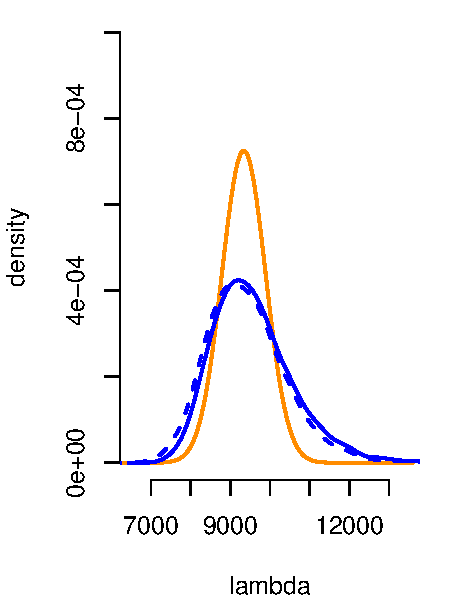
\includegraphics[width=.34\textwidth]{graphs/tail33203-u9000-a1-b1.pdf}\!\!\!\!\!\!\!
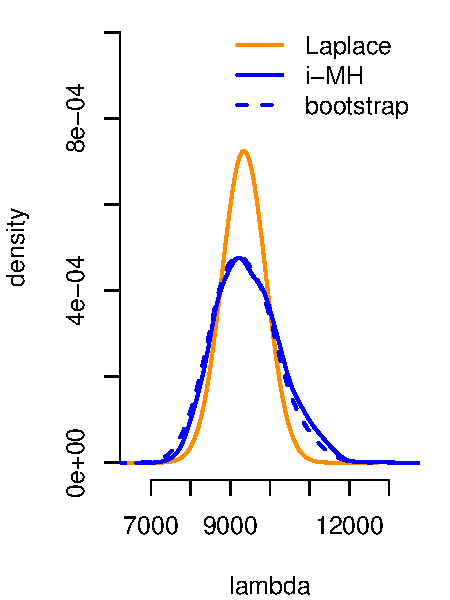
\includegraphics[width=.34\textwidth]{graphs/tail33203-u9000-a9-b9.pdf}\!\!\!\!\!\!\!
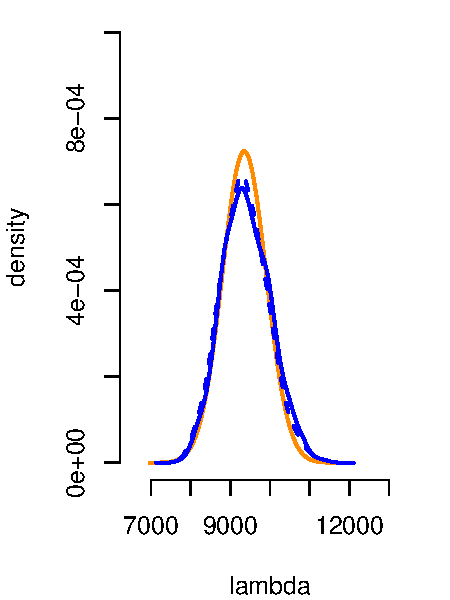
\includegraphics[width=.34\textwidth]{graphs/tail33203-u9000-a80-b80.pdf}
\end{center}

These results give all we need for  inference about the overall mean.

\end{frame}

\begin{frame}


Performance over 200 resamples
of $N=50,000$ from $10^7$ total. 

\begin{center}
\includegraphics[width=.85\textwidth]{graphs/performance-avg-50000.pdf}\\
{\scriptsize
\bf ~~~~~{\color{DarkBlue} -- Bayes a,b=1} \hspace{.5cm} {\color{DodgerBlue} -- Bayes a,b=9} \hspace{.5cm}{\color{LimeGreen} -- Bayes a,b=80} \\{\color{Pink} -- Winsorization} \hspace{.3cm}{\color{red} --  FW tilting} \hspace{.3cm} {\color{black!70} -- sample mean} \hspace{.3cm} {\color{Gold} -- N/2 subsampling} }
\end{center}

% Lowest-possible RMSE + accurate frequentist coverage,
% and fast!
\vskip -.5cm
\end{frame}

\begin{frame}
{\bf Consistency and thresholds}

The \textit{semiparametric bootstrap}  is consistent if 
$u_N = O(N^{\xi/(1+2\delta\xi)})$. \\ {\gr Which is cool, because the nonparametric bootstrap is not.}

\vskip .5cm
In this limit, $\sigma_N = \xi u_N$.  So, one can increase $u$ until this  holds. { Indeed, it  holds roughly in our examples for good performing $u$.}

\vskip  .5cm
In practice, {\theme results are robust to a range of tail thresholds}. 

\vskip .5cm {This also suggests why informative priors on $\sigma$ are not useful:\\~~ it is already informed by both the threshold and the tail index.}

\end{frame}

\begin{frame}
{Semi-parametrics in treatment effect estimation}


Semiparametric inference makes a big difference in A/B analysis.\\
 Looking at ATEs, $\mu_1 - \mu_2$, in a few example experiments:

\vskip .25cm
\hfill {\footnotesize {\bl sp-bayes}, {\bk capped}, {\rd naive}}
\begin{center}
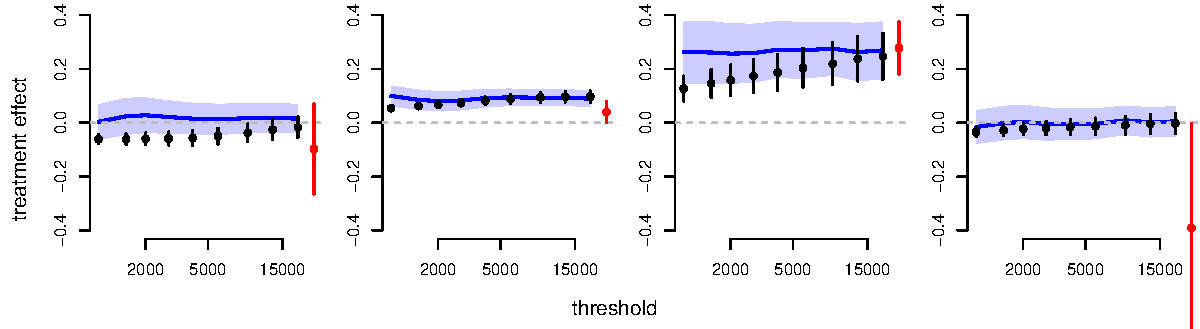
\includegraphics[width=\textwidth]{graphs/ABtrials}
\end{center}

\vskip -.25cm
Such care in uncertainty quantification is essential whenever you need to understand the full posterior (or sampling) distribution. {\gr e.g., bandit learning with heavy-tailed rewards is another application.\!\!\!}
\vskip -.25cm
\end{frame}

\begin{frame}


{\bf Efficient Big Data analysis}


\vskip .25cm 
We're reserving difficult modeling for the difficult parts of our learning problem, while taking advantage of nonparametric consistency and large numbers of observations for the easy bits

\vskip .25cm
In general, we statisticians and machine trainers should be thinking about what portions of the `model' are {\theme hard} or {\nv easy} to learn.

\vskip .25cm
Once we figure this out,  we can use a little bit of the data to\\ learn the easy stuff and direct our full data at the hard stuff.

\vskip .25cm
This is {\it the} future for Big Data.

\hfill \huge \theme \bf thanks!

\end{frame}



\end{document}






























